% Modelo Desenvolvido no decorrer do Projeto  
% LaTeX para Instituições de Ensino Superior CM 
% Coordenadores: Professor Dr. Adilandri Mércio Lobeiro 
%                Professor Dr. Marco Aurélio Graciotto 
% Bolsista Do Projeto: Discente: Rafael Rampim Soratto 
 
\documentclass{modelo}
\usepackage[brazil]{babel}     
%\usepackage[english]{babel}  
\usepackage[utf8]{inputenc}   
%\usepackage[utf8]{fontenc}
\usepackage{amsmath,amsfonts,amssymb}
\usepackage{graphicx,graphics} 
\usepackage{xcolor} 
%\usepackage{ifthen}
\usepackage{float} 
\usepackage{fancyhdr} 
\usepackage[font={small}]{caption}  
\usepackage{array} 
\usepackage{lastpage}
\usepackage[square]{natbib} 
\bibliographystyle{abbrvnat}
\setlength\bibhang{0cm}   
\usepackage{verbatim}
    
  
\pagestyle{fancy}   
 
 
  
\fancypagestyle{sei}{   
\pagestyle{plain}	
%\fancyhf{} 
\fancyhead{} 
\fancyfoot{}   	
\lhead{     	

\includegraphics[scale=0.34]{figs/seii}  
\textcolor{black}{\textbf{\Large VIII SEI}} 	 
}   
\rhead{ $8^\circ$ Seminário de Extensão e Inovação}
 
\lfoot{\small{\textcolor{black}{\small{\textbf{página}}} \thepage \textbf{\color{black}de} \pageref{LastPage}}}  
\rfoot{\small{Seminário de Extensão e Inovação, 8., 2018, Apucarana, PR.}} 
  
\renewcommand{\headrulewidth}{2pt} 
\renewcommand{\footrulewidth}{2pt}  
 
}   
 

%************ INSIRA OS DADOS DO SEU TRABALHO A PARTIR DAQUI *********     
% 
% O resumo deve ter 250 palavras no máximo.  
% e de preferência deve possuir os 4 tópicos: Objetivos, métodos, resultados e conclusão.
 
\newcommand{\resumotexto}  
{  
%\textbf{Objetivos:} \objetivos \
%\textbf{Métodos:} \metodos  
%\textbf{Resultados:} \resultados \
%\textbf{Conclusão:} \conclusao	 
   
O objetivo destas instruções é que sejam usadas como um modelo para a formatação de trabalhos que serão submetivos ao XXIII SCITE. O reseumo deve descrever os objetivos do trabalho, a metodologia de uma forma condensada e as conclusões principais em um intevalo de 100 a 250 palavras.    
É importante ressaltar que não devem estar presentes no resumo fórmulas e referências bibliográficas.O resumo será publicado nos Anais do evento quando o trabalho for selecionado para pôster e o resumo expandido será publicado caso o mesmo seja selecionado para apresentação oral.
%O título desta seção deve ser redigido em fonte Times New Roman, tamanho 11, em letras maiúsculas e centralizadas. \\  
O texto do resumo deveapresentar fonte de tamanho 10 e alinhamento justificado. Os nomes dos autores devem ser posicionados à esquerda do resumo, em letras maiúsculas,fonte de tamanho 8, seguido do endereço de email a baixo, filiação por extenso, cidade, estado e pais. As palavras chave devem ser apresentadas na sequência, com fonte de tamanho 0, com no máximo 5 palavras.
}

% Palavra chave deve ser separada por ponto e ter apenas de 3 a 5 palavras:
 
\newcommand{\palavraschave}{Palavra um. Palavra dois. Palavra três. Palavra quatro. Palavra cinco (até 5). } 
 
\newcommand{\agradecimentosTexto}{Esta seção é obrigatória aos trabalhos que receberam bolsa e auxílio financeiro. Deve apresentar os agradecimentos aos principais órgãos de fomento (bolsa e auxílio financeiro), instituições e pessoas que contribuíram para a realização do trabalho. Não exceder 50 palavras e alocá-los antes das referências.}
\newcommand{\kwords}{KeyOne. KeyTwo. KeyT.} 
\newcommand{\resumoingles}{
	The objective is to be short, defining the problem studied, highlighting the knowledge gaps that are addressed in any article.
	Data sources, a sample studied, a sampling, a selection pattern, analytical procedures, among others, should be fully and completely answered. In order to obtain complete results, the results can be included in the interpretations or comparisons. A conclusion of the authors on the results that appear and on their implications.}  	
%********************************************************
% Título 
	
\begin{document}

 	
\title{Modelo para a formatação dos resumos expandidos a serem submetidos ao \Rnth{23} Seminário de Iniciação Científica e Tecnológica da UTFPR(SICITE)} 

 
  	 
\author{  
 
% Editar nome e email de autores para o título do texto. 
% Todo autor deve ter universidade e local.   
% Não usar abreviaturas em nomes.
% Para adicionar autores de alguma universidade: 
% \criarautor{Nome}{e-mail} 

\criarautor{Rafael Soratto}{email@hotmail.com}{ Universidade Tecnológica Federal do Paraná - (UTFPR), Campo mourão, PR, Brasil.\\} 
\criarautor{Adilandri Mércio Lobeiro}{adilandri@gmail.com}{ Universidade Tecnológica Federal do Paraná - (UTFPR), Campo mourão, PR, Brasil.\\} 

% Comando para adicionar a universidade dos autores a cima :  
% \criaruniversidade 
%  {Nome da universidade, (SIGLA), Cidade, Estado, Pais }
%\criaruniversidade{ Universidade Tecnológica Federal do Paraná - (UTFPR), Campo mourão, PR, Brasil.}  
 
 
% Outro exemplo:
%\criarautor{Nomex}{emailx},  
%\criarautor{Nomey}{emaily}  

	  
% Indica que os três autores acima são da mesma universidade(Universidade-sigla-estado-país):	 

%\criaruniversidade{Universidade Estadual de Maringá - (UEM), Maringá, PR,   Brasil.}
			 
% Final do Título 
} 
  
%********************************************************  
% Pré-Textual	 

% Nada do Pré-Textual e Pós Textual devem ser alterados!   

\criartitulo  
\thispagestyle{plain}  
\pagestyle{plain}
 
 
	


 
 %*********************************************************
% Textual : 
 
 % Alterar a partir daqui: 
  
 \section{Introdução}
 
 Da introdução, até o final da conclusão, de 2 a 4 páginas. Os trabalhos devem ser redigidos na ortografia oficial e digitados em folhas de papel tamanho A4. Os trabalhos deverão conter: 
 \begin{itemize}
     \item[No minímo] duas páginas; 
      \item[No máximo] quatro páginas;
 \end{itemize}
   Sugere-se digitar o trabalho no progama Word para Windows e converter o arquivo em PDF para submissão ou com \LaTeX. Desta forma não haverá problemas de formatação por incompatibilidade de versões de progamas. A comissão científica também disponibilizará o template para trabalhos redigidos em \LaTeX. Não serão aceitos para avaliação resumos expandidos em outro formato. Sugere-se a utilização deste arquivo para digitar o trabalho. 
   
 \section{Formato do Texto} 
 No corpo do texto, o testo deve iniciar na linha abaixo do título das seções. Os trabalhos devem ser redigidos em Português, usando fonte Times New Roman, tamanho 11, exceto para o título., filiação dos autores, resumo e palavras-chave. Deve ser aplicado espaçamento simples entre as linhas de todo o trabalho.
 
 Os títulos das sessões devem ser posicionados à esquerda e sem ponto final. As páginas devem ser numeradas na parte inferior à esquerda conforme o modelo deste documento.
  
  O corpo do texto deve ser justificado, sen a primeira linha de cada parágrafo deslocada meio centímetro. AS referências utilizadas ao longo do trabalho devem ser listadas no final do trabalho de acordo com as instruções da seção "Referências".
 
 Aspas devem ser utilizadas somente em citações diretas. Negrito deve ser utilizda para dar ênfase a termos, frase ou símbolos. Itálico deverá ser utilizado apenas para palavras em língua estrangeira(e.g.\textit{for exemple}).
 
 No caso de uso de alíneas obedecer às seguintes indicações: 
 
 \begin{itemize}
     \item[(a)] cada item da alínea deve ser ordenado alfabeticamente por letras mínusculas seguidas de parênteses; 
     \item[(b)] os itens da alínea são separados entre si por ponto e vírgula; 
     \item[(c)] a estrutura dos resumos expandidos é a convencial: Introdução, Métodos, Resultados, Discussão e Considerações Finais; 
     \item[(c)] o último item de alínea termina com ponto.
 \end{itemize}
\textbf{Notas:} as notas devem ser evitadas.
 
 \subsection{Títulos em Seções Secundárias} 
 Os títulos das seções secundárias devem se apresentar em letras maiúsculas e sem ponto final. Devem estar alinhadas à esquerda, em fonte Times New Roman 11 e em negrito. 
  

  
\subsection{Figuras, Quadros e Tabelas}  

Qualquer que seja o tipo de ilustração inserida no trabalho(fluxograma, gráfico, quadro, figura,imagem,tabela,entre outros) sua identificação deve aparecer na parte superior, precedida da palavra designitiva, seguida de seu número de ordem de ocorrência no texto, em algarismos arábicos, travessão e do respectivo título e com fonte de tamanho 10. Após a ilustração ou tabela, na parte inferir, indicar a fonte consultada(mesmo sendo de produção do própio autor)
A ilustração deve ser citada no texto e inserida o mais próximo possível do trecho a que se refere. ver, por exemplo, a \ref{fig:figura1}


\begin{figure}[H] 
\begin{center} 
\label{fig:figura1}  
\caption{Figura}
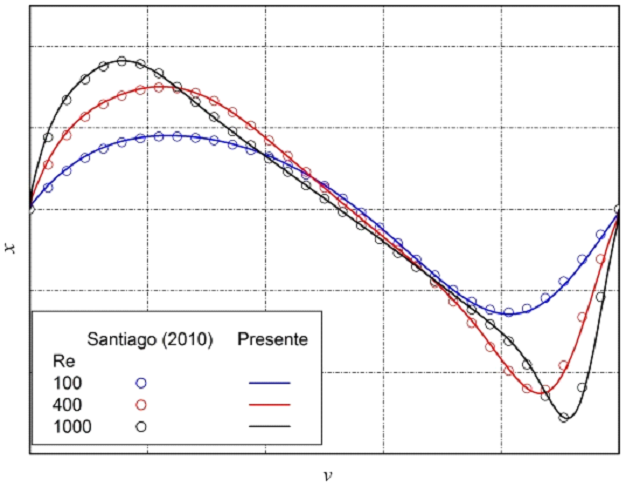
\includegraphics[scale=0.5]{figs/fig1} \\
\textbf{Fonte: Autoria Própria (2018)}
\end{center}
\end{figure}

Tabelas e quadros devem estar centralizados e conter apenas dados imprescindíveis, evitando-se que sejam muito extensos, não repetindo dados já inseridos no texto, ou vice-versa. O formato pode ser observado na Tabela 1. 

No caso de quadros, deve ser seguida a estrutura demonstrada no Quadro 1. Caso os dados sejam inéditos e provenientes de uma pesquisa realizada pelos próprios autores do trabalho, essa especificação deve constar na fonte com o ano da pesquisa de campo. Nesse caso a fonte deve ser: Autoria própria (2017). 
  
 \subsection{Equações Matemáticas} 
 As equações matemáticas devem aparecer a partir de um deslocamento de 0,5 cm a partir da margem esquerda, em fonte Times New Roman tamanho 10. Números arábicos devem ser usados em equações, inseridos entre parênteses, como ilustrado na Equação \ref{equation:eq1}.  
  
  \begin{equation}
      u = \beta \sin{\left ( \pi x \right )}\frac{\left ( e^{2x}-1 \right ) \left ( e^{y}-1 \right )}{\left ( e^{2}-1 \right ) \left ( e-1 \right )} 
      \label{equation:eq1}
  \end{equation} 
   
 
 
 \section{Citações e Referências} 
 
 As citações devem obedecer ao sistema autor-data e estar de acordo com a norma NBR 10520 da Associação Brasileira de Normas Técnicas (ABNT). 
Citações diretas de até três linhas acompanham o corpo do texto e se destacam com aspas duplas. Caso o texto original já contenha aspas, estas devem ser substituídas por aspa simples.   

Exemplos:
 
Fulano (2008, p. 10) afirma que “[...] é importante a utilização das citações corretamente”.
"Citar trechos de ‘outros autores’ sem referenciá-los, pode ser caracterizado plágio” (FULANO; BELTRANO, 2009, p. 20, grifo do autor). 

Para as citações com mais de três linhas, estas devem ser transcritas em parágrafo distinto. Exemplo:    
\begin{citacao}
Toda citação direta com mais de 03 linhas é considerada uma citação direta longa. A citação com mais de 03 linhas deve ser escrita sem aspas, em parágrafo distinto, com fonte de tamanho 10, espaçamento simples e com recuo de 4,0 cm da margem esquerda, terminando na margem direita, conforme ilustrado neste exemplo (FULANO, 2009, p. 150).  
\end{citacao} 

 A exatidão das referências é de responsabilidade dos autores e devem ser elaboradas de acordo com a NBR 6023 da ABNT. 
Todas as referências citadas no texto, e apenas estas, devem ser incluídas ao final, na seção Referências. 
As referências devem incluir apenas aquelas centrais e relevantes à problemática abordada. É, também, desejável que se evite a utilização de livros, priorizando os periódicos como referência. 

Todas as obras consultadas que estiverem disponíveis na internet devem ser referenciadas com o endereço eletrônico e data de acesso. 

%\noindent\fbox{\begin{minipage}{\dimexpr\textwidth-2\fboxsep-2\fboxrule\relax}
%		\centering
%	\begin{tabular}{|c|c|c|}
%		\hline 
%		Seção & Tipografia & Exemplo \\ 
%		\hline 
%		Seções Primárias & Letras Maiúsculas em negrito   & \textbf{1 Seção Primária} \\ 
%		\hline 
%		Seções Secundárias &  &  \\ 
%		\hline 
%		Seções Terciárias &  &  \\ 
%		\hline 
%	\end{tabular} 
%	
%\end{minipage}} 
%
%\begin{mdframed}
%	If A and B are two events that are not mutually exclusive then: 
%	\[ 
%	P(A \cup B) = P(A) + P(B) - P(A \cap B) 
%	\] 
%\end{mdframed}
%
%\bigskip
%\begin{mdframed}[
%	linecolor=teal,linewidth=2pt,% 
%	frametitlerule=true,% 
%	apptotikzsetting={\tikzset{mdfframetitlebackground/.append style={%
%				shade,left color=white, right color=blue!20}}}, 
%	frametitlerulecolor=teal,
%	frametitlerulewidth=1pt, innertopmargin=\topskip,
%	frametitle={Non Mutually Exclusive Events},
%	outerlinewidth=1.25pt
%	]
%	% ----------
%	If A and B are two events that are not mutually exclusive then: 
%	\[ 
%	P(A \cup B) = P(A) + P(B) - P(A \cap B) 
%	\] 
%\end{mdframed}   
% 
% \begin{tcolorbox}[skin=widget,
% 	boxrule=1mm,
% 	coltitle=black,
% 	colframe=teal,
% 	colback=white,
% 	width=(.9\linewidth),before=\hfill,after=\hfill,
% 	adjusted title={ }]
% 	If A and B are two events that are not mutually exclusive then:  
%
% 	$P(A \cup B) = P(A) + P(B) - P(A \cap B)$
% \end{tcolorbox} 
     
 
%*********************************************************** 
% Pós-Textual  

% Pós e Pre Textuais não devem ser alterados, porém as macros que terminam com "Texto" devem ser preenchidas no preâmbulo.

\titleformat{\section}{\normalfont} 
{\thesection}{14pt}{\bfseries\Large}  

\newpage  

\begin{abstractt}  
\resumoingles 
\end{abstractt}   
\begin{keywordss}
\kwords
\end{keywordss}

\section*{Agradecimentos}
\thanks{\agradecimentosTexto}  

%\section*{Referências Bibliográficas}  
\bibliography{sei-template-bib} 


%\appendix
%\section*{Apêndice, ou complementos (Opcional!)}\label{apendiceA}
%%IMPORTANTE
%%Aqui são incluídas informações complementares, se necessárias; caso contrário RETIRE todo 
%%esse texto. Não esquecer de deixar o comando \end{document} que encontra-se na última linha do arquivo.


\end{document}
